\documentclass[11pt,a4paper]{article}
\usepackage[top=0in, bottom=0.5in,margin=1in, includefoot]{geometry}
\usepackage[utf8]{inputenc}
\usepackage[T1]{fontenc}
\date{}
\author{}
\setlength\parindent{0pt}
\usepackage{amsmath}
\usepackage{wrapfig}
\usepackage{graphicx}
\usepackage{lineno}
\usepackage{layout}
\usepackage{alltt}
\usepackage[justification=centering]{caption}
\usepackage[export]{adjustbox}
\usepackage{ulem}
\usepackage{subcaption}
\usepackage[section]{placeins}

\setlength{\voffset}{-0.4in}
\textheight = 735pt
\begin{document}
\vspace{-20mm}
\title{\textbf{EE2-08C Numerical Analysis} \\ Group 9\vspace{-17mm}}
\maketitle
\tableofcontents
\pagebreak

\section{Exercise 1 - RL Circuit}\vspace{-1mm}

\subsection{Background}
\begin{wrapfigure}{r}{0.5\textwidth}
\vspace{-10mm}
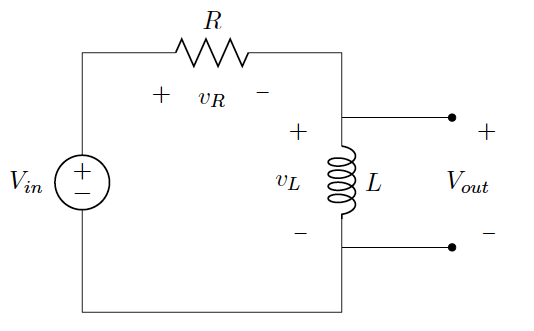
\includegraphics[width=0.49\textwidth]{Ex1_Figs/RL_circuit.png}
\vspace{-6mm}
\caption{RL Circuit}
\label{fig:RL1}
\end{wrapfigure}
This simple RL circuit (\ref{fig:RL1}) forms a high pass filter circuit which takes an input signal Vin and only allows the high frequency components to pass. Despite the inductor being less convenient than a capacitor, this RL circuit can approach the model of a DC motor. In this specific case, we want to model a DC motor with inertia 250 $\mu$sNm/s$^2$ and $T_{max} = 50mNm/A$. To do so, according to KCL, we know that

\begin{equation}
Vin(t) = v_L(t) + v_R(t)
\end{equation}


and therefore:
\begin{equation}
V_{in}(t) = L\frac{d}{dt}i_L(t) + R i_L(t)
\end{equation}

$i_L(t)$ is the state that we will solve following the three different second-order Runge Kutta methods.

All methods follow the same pattern:
\begin{equation}
x_{i+1} = x_i + h
\end{equation}

$h$ being the step size and
\begin{equation}
   y_{i+1} = y_i + h (a k_1 + b k_2)
\end{equation}

where

\[k_1 = f(x_i, y_i)\]
\[k_2 = f(x_i + p h, y_i + q k_1 h)\]

and the values of $a, b, p$ and $q$ depend on which method we are using:

\begin{center}
 \begin{tabular}{||c | c c c||}
 \hline
 Parameter & Heuns & Midpoint & Ralston \\ [0.5ex]
 \hline\hline
 a & 1/2 & 0 & 1/4 \\
 \hline
 b & 1/2 & 1 & 3/4 \\
 \hline
 p & 1 & 1/2 & 2/3 \\
 \hline
 q & 1 & 1/2 & 2/3 \\ [1ex]
 \hline
\end{tabular}
\end{center}

Each method will approximate the exact solution according to these parameters. Therefore, the smaller the step size $h$, the more exact the method will approximate the solution.

 After doing so, the output value will be obtained as follows:
\begin{equation}
V_{out} = V_{in}(t) - R i_L(t)
\end{equation}

\newpage

\subsection{Second-Order Runge Kutta Scripts}

\vspace{-2mm}The code for Heuns.m to solve $i_L(t)$ will be as follows:

\begin{verbatim}
function [t,y] = heun(func,t0,y0,tf,h) % y = i_L(t), func = equation (2),
% t0 = initial time, tf = final time, h = step size
N = round((tf-t0)/h);   % N = nr. of steps
arrt = zeros(1,N);      % arrt = array of time
arry = zeros(1,N);      % arry = array of y
arrt(1) = t0;           % initial conditions
arry(1) = y0;
for i = 1 : N-1         % evaluate arry and arrt for each step
    k1 = feval(func, arrt(i), arry(i));
    k2 = feval(func, arrt(i) + h, arry(i) + k1*h);
    arry(i+1) = arry(i) + h*0.5*(k1 + k2);
    arrt(i+1) = arrt(i) + h;
end
t= arrt;                % return values
y = arry;
end
\end{verbatim}

\vspace{-2mm}Similarly, the code for Midpoint.m will be:
\vspace{-1mm}
\begin{verbatim}
function [t,y] = midpoint(func, t0, y0, tf, h)     % y = i_L(t), func = equation (2),
% t0 = initial time, tf = final time, h = step size
N = round((tf - t0)/h); % N = nr. of steps
arrt = zeros(1,N);      % arrt = array of time
arry = zeros(1,N);      % arry = array of y
arrt(1) = t0;           % initial conditions
arry(1) = y0;
for i = 1:N-1           % evaluate arry and arrt for each step
    k1 = feval(func,arrt(i),arry(i));
    k2 = feval(func, arrt(i) + 0.5*h, arry(i) + 0.5*h*k1);
    arry(i+1) = arry(i) + h*((1/4)*k1 + (3/4)*k2);
    arrt(i+1) = arrt(i) + h;
end
t = arrt; y = arry;     % return values
end
\end{verbatim}

Lastly, Ralston.m will be as similar:

\begin{verbatim}
function [t, y] = ralston(func,t0,y0,tf,h)  % y = i_L(t), func = equation (2),
% t0 = initial time, tf = final time, h = step size
N = round((tf-t0)/h);   % N = nr. of steps
arrt = zeros(1,N);      % arrt = array of time
arry = zeros(1,N);      % arry = array of y
arrt(1) = t0;           % initial conditions
arry(1) = y0;
for i = 1 : N-1         % evaluate arry and arrt for each step
    k1 = feval(func, arrt(i), arry(i));
    k2 = feval(func, arrt(i)+(2/3)*h, arry(i)+(2/3)*h*k1);
    arry(i+1) = arry(i) + (h/4)*(k1 + 3*k2);
    arrt(i+1) = arrt(i) + h;
end
y = arry; t = arrt;     % return values
end
\end{verbatim}

As mentioned above, we can appreciate that the three second-order Runge Kutta methods are almost identical with the parameters inside the $for$ $loop$ the only difference between them.

\newpage
\subsection{Script to solve the ODE}
Given that the values of the components of the RL circuit are:

\[R = 0.5\Omega\ \hspace{3mm} L = 1.5mH\]

We will find the value of $V_{out}$ according to a script which always follows the same pattern, depending on the values of $V_{in}$ and adjusting the values of $h$ and $t_f$. A standard script would be as follows:

\begin{verbatim}
y0 = 0;
t0 = 0; tf = ***;   % to decide
h = ***;            % to decide

Vin =@(t) ***;      % different inputs

R = 0.5; L = 1.5*10^(-3);           % R, L values for this project
func =@(t, y) (Vin(t) - R*y)/L;     % equation 2
[t, y] = ****(func,t0,y0,tf,h);     % heuns, midpoint or ralston
vout = Vin(t)-R*y;                  % equation 5
figure;
plot(t, vout);      % plot V_out against time
title '****'
xlabel 't(s)'
ylabel 'Vout(t)'

\end{verbatim}
\newpage
\subsection{Exercise 1 - Graphs}
\subsubsection{Step signal with amplitude}
\begin{wrapfigure}{r}{0.5\textwidth}
        \vspace{-15mm}
        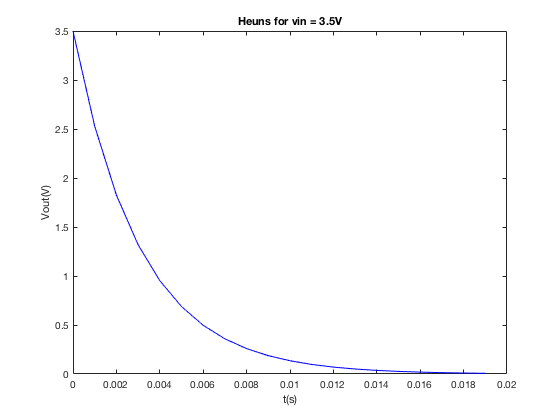
\includegraphics[width=0.49\textwidth]{Ex1_Figs/heuns_step.png}
        \vspace{-6mm}
        \caption{Heuns for Vin = 3.5V}
        \label{fig:RL2}
    \end{wrapfigure}

$\tilde{V}_{in} = 3.5V$ \\
    $t0 = 0$, $tf = 0.02$; \\
    $h = 0.001$; \\
    $Vin = @(t) 3.5$; \\
    %$[t,y] = heuns(func, t0, y0, tf, h)$ \\

In the step signal case, all methods will lead to equal approximation of the solutions. Figure \ref{fig:RL2} is applying Heuns method, but if we apply Midpoint (Figure \ref{fig:RL3}) or Ralston (Figure \ref{fig:RL4}) with the same step size and time conditions, we get similar plots.


\begin{figure}[b]
	\begin{subfigure}{.5\textwidth}
  		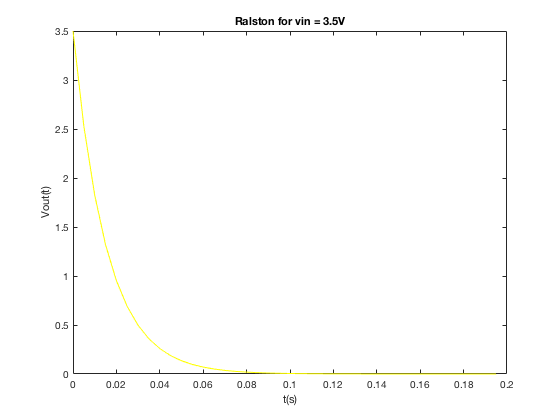
\includegraphics[width=.9\linewidth,height = 5cm]{Ex1_Figs/ralston_step.png}
  		\caption[right]{Ralston for Vin = 3.5V}
  		\label{fig:RL4}
	\end{subfigure}
	\begin{subfigure}{.5\textwidth}
  		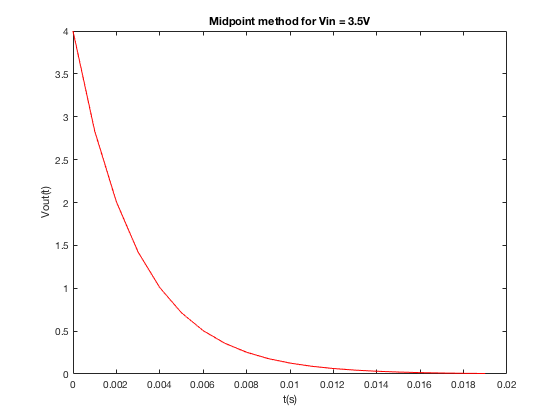
\includegraphics[width=.9\linewidth,height = 5cm]{Ex1_Figs/midpoint_step.png}
  		\caption{Midpoint for Vin = 3.5V}
  		\label{fig:RL3}
	\end{subfigure}
	\caption{Ralston and Midpoint for Vin = 3.5V}
	\label{fig:test}
\end{figure}

\pagebreak

The MATLAB code below is used to plot teh result from all three methods on one graph (Figure \ref{fig:RL5}).

\begin{verbatim}
    [t,y] = heun(func,t0,y0,tf,h);
    Vout = Vin(t) - R*y;
    figure;
    plot(t, Vout, 'b'); % plot heuns method in blue
    hold on;
    [t,y] = ralston(func,t0,y0,tf,h);
    Vout = Vin(t) - R*y;
    plot(t, Vout, 'r')  % plot midpoint method in red
    hold on;
    [t,y] = ralston(func,t0,y0,tf,h);
    Vout = Vin(t) - R*y;
    plot(t, Vout, 'g')
    title 'All for step signal Vin = 3.5V'
    xlabel 't(s)'
    ylabel 'Vout(V)'
    legend ('Heuns', 'Midpoint', 'Ralston')
    \end{verbatim}

  \begin{figure}[h]
    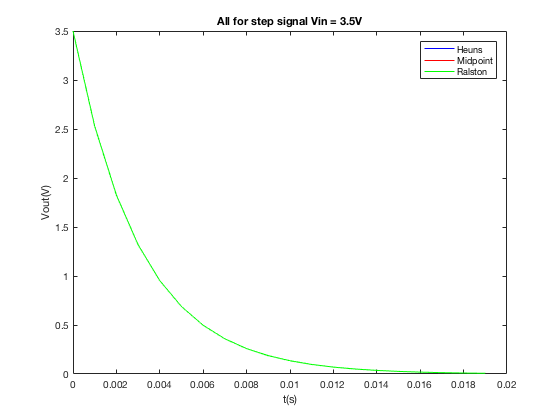
\includegraphics[width=0.49\textwidth,center]{Ex1_Figs/all_step.png}
    \caption{All for Vin = 3.5V}
    \label{fig:RL5}
    \end{figure}
 The code above was used to plot all three methods on the same graph. The plot (Figure \ref{fig:RL5}) proves that the three methods are equal for the same step size and time conditions for the given input (Vin = 3.5V).


\newpage
\subsubsection{Impulsive signal and decay}
$Vin = Vin*exp(-t^2/\tau)$

\begin{wrapfigure}{r}{0.5\textwidth}
\vspace{-15mm}
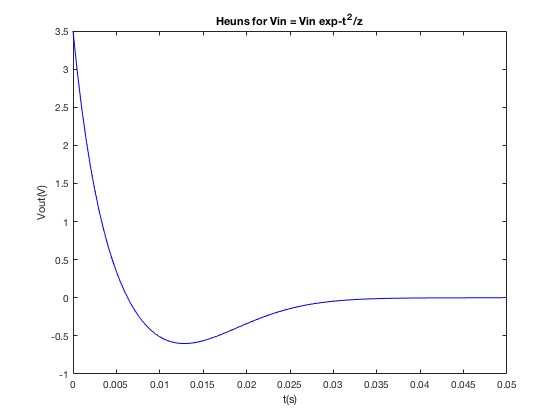
\includegraphics[width=0.49\textwidth,center]{Ex1_Figs/heun_t2.png}
\vspace{-6mm}
\caption{Heuns for $Vin = Vin*exp(-t^2/\tau)$}
\label{fig:RL6}
\end{wrapfigure}

In this section, we will examine the 2nd order Runge Kutta Methods using an impulsive signal input given in the equation below:

 \begin{equation}
V_{in} = \tilde{V}_{in}  exp{-t^2/\tau}
\end{equation}

 \begin{verbatim}
    t0 = 0, tf = 0.05;
    h = 0.0005;
    vin = 3.5;
    z = 150*10^(-6);
    t = t0: T : tf;
    Vin = @(t) vin*exp(-(t.^2)/z)
    \end{verbatim}

\begin{figure}[h]
\begin{subfigure}{.5\textwidth}
  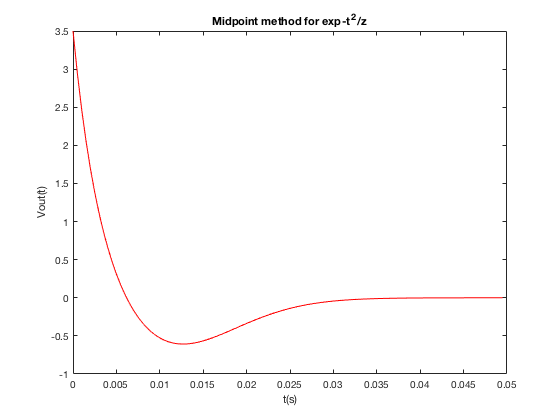
\includegraphics[width=.9\linewidth,height = 5cm]{Ex1_Figs/mid_t2.png}
  \caption[right]{Midpoint for $Vin = Vin*exp(-t^2/\tau)$}
  \label{fig:RL7}
\end{subfigure}
\begin{subfigure}{.5\textwidth}
  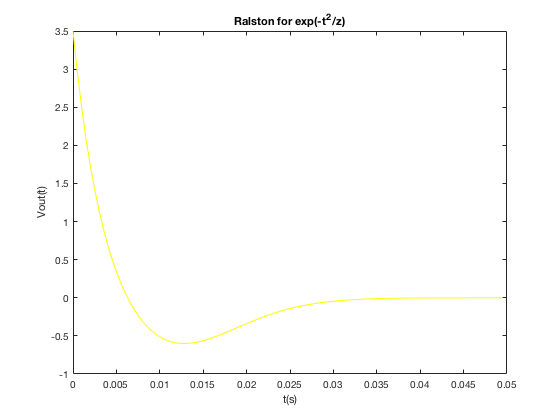
\includegraphics[width=.9\linewidth,height = 5cm]{Ex1_Figs/ral_t2.png}
  \caption{Ralston for $Vin = Vin*exp(-t^2/\tau)$}
  \label{fig:RL8}
\end{subfigure}
\caption{Ralston and Midpoint for $Vin = Vin*exp(-t^2/\tau)$}
\label{fig:RLx}
\end{figure}


%Put comments on figures 5 and 6 here

\newpage
$Vin = Vin*exp(-t/\tau)$

\begin{wrapfigure}[0]{r}{0.5\textwidth}
\vspace{-30mm}
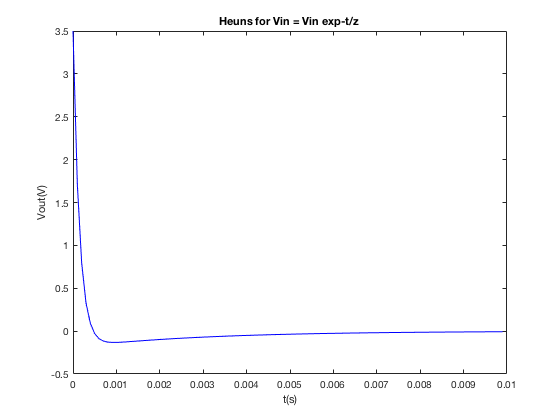
\includegraphics[width=0.49\textwidth,center]{Ex1_Figs/heuns_t.png}
\vspace{-6mm}
\caption{Heuns for $Vin = Vin*exp(-t/\tau)$}
\label{fig:RL9}
\end{wrapfigure}

In order to examine the behaviour of the three 2nd order Runge Kutta methods, we will demonstrate their outputs with another impulsive signal given below:


$V_{in} = \tilde{V}_{in}  exp{-t/\tau}$

\begin{verbatim}
t0 = 0; tf = 0.1;
h = 0.001;
vin = 3.5;
z = 150*10^(-6);
t = t0: T : tf;
Vin = @(t) vin*exp(-(t)/z);
\end{verbatim}

\begin{figure}[h]
\begin{subfigure}{.5\textwidth}
  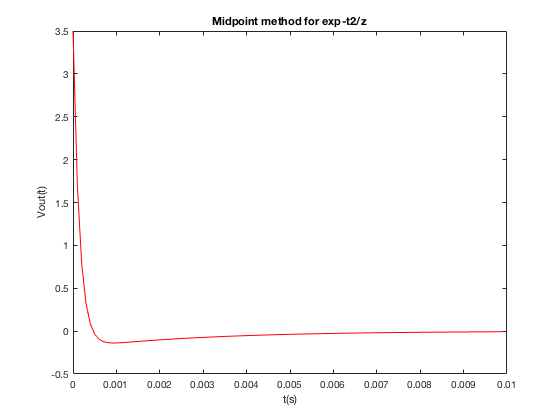
\includegraphics[width=.9\linewidth,height = 5cm]{Ex1_Figs/mid_t.png}
  \caption[right]{Midpoint for $Vin = Vin*exp(-t/\tau)$}
  \label{fig:RL10}
\end{subfigure}
\begin{subfigure}{.5\textwidth}
  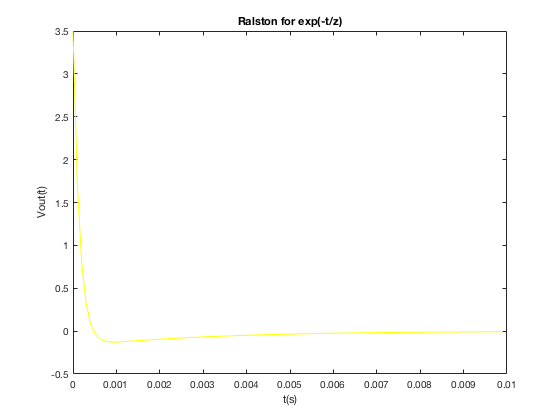
\includegraphics[width=.9\linewidth,height = 5cm]{Ex1_Figs/rals_t.png}
  \caption{Ralston for $Vin = Vin*exp(-t/\tau)$}
  \label{fig:RL11}
\end{subfigure}
\caption{Ralston and Midpoint for $Vin = Vin*exp(-t/\tau)$}
\label{fig:RLy}
\end{figure}


For both impulsive signals, the difference in the outputs obtained from the three different methods between  is minimal. This can be seen from the graphs in Figure:\ref{fig:RL12} and Figure: \ref{fig:RL13} which plot all three curves obtained for the two impulsive signal inputs $V_{in} = \tilde{V}_{in}  exp{-t^2/\tau}$ and $Vin = Vin*exp(-t/\tau)$ respectively.

\begin{figure}[h]
\begin{subfigure}{.5\textwidth}
  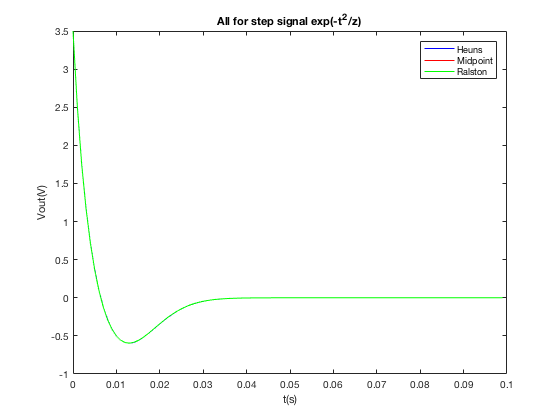
\includegraphics[width=.9\linewidth,height = 5cm]{Ex1_Figs/all_t2.png}
  \caption[right]{All for $Vin = Vin*exp(-t^2/\tau)$}
  \label{fig:RL12}
\end{subfigure}
\begin{subfigure}{.5\textwidth}
  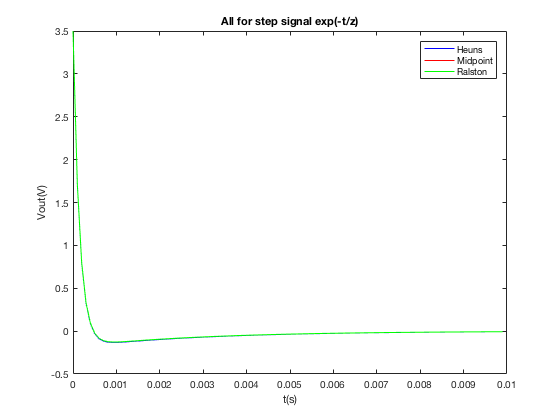
\includegraphics[width=.9\linewidth,height = 5cm]{Ex1_Figs/all_t.png}
  \caption{All for $Vin = Vin*exp(-t/\tau)$}
  \label{fig:RL13}
\end{subfigure}
\caption{All for $Vin = Vin*exp(-t/\tau)$ and $Vin = Vin*exp(-t^2/\tau)$}
\label{fig:test3}
\end{figure}

\newpage
\subsubsection{Sine wave amplitude $\tilde{V}_{in} = 4V$}

For the waves cases, three methods will be plot in the same graph for comparison purposes and avoid overloading of graphs.

\begin{verbatim}
vin = 4;
T = ***10^(-6);
t = t0: T : tf;
f = 1/T;
Vin =@(t) vin*sin(2*pi*f*t);
\end{verbatim}

\begin{figure}[h]
\begin{subfigure}{0.5\textwidth}
\centering
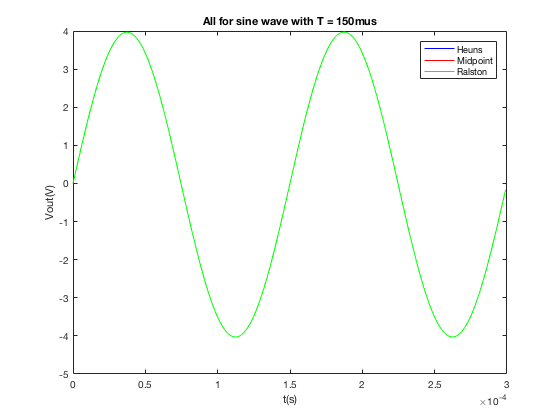
\includegraphics[width=.8\linewidth]{Ex1_Figs/allsine150g.png}
\caption{$T = 150\mu s$,  $h = 0.000001$  and $t_f = 0.003$}
\label{fig:sfig1}
\end{subfigure}
\begin{subfigure}{0.5\textwidth}
\centering
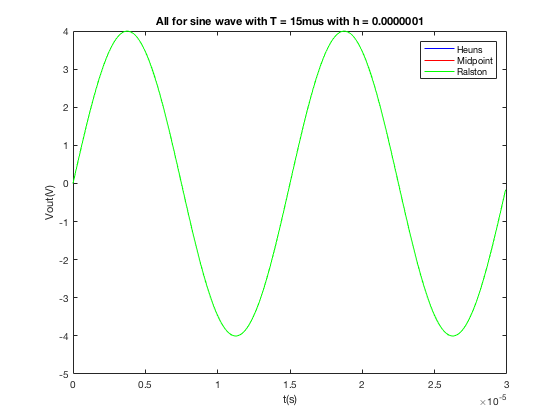
\includegraphics[width=.8\linewidth]{Ex1_Figs/allsine15g.png}
\caption{$T = 15\mu s$, h = 0.0000001 and tf = 0.00003}
\label{fig:sfig2}
\end{subfigure}
\begin{subfigure}{.5\textwidth}
\centering
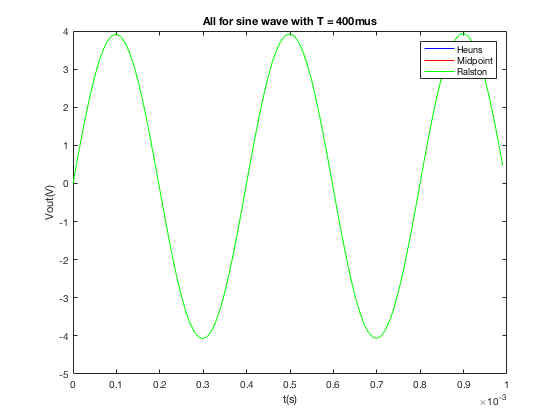
\includegraphics[width=.8\linewidth]{Ex1_Figs/allsine400.png}
\caption{$T = 400\mu s$,  $h = 0.00001$ and $t_f = 0.001$}
\label{fig:sfig3}
\end{subfigure}
\begin{subfigure}{0.5\textwidth}
\centering
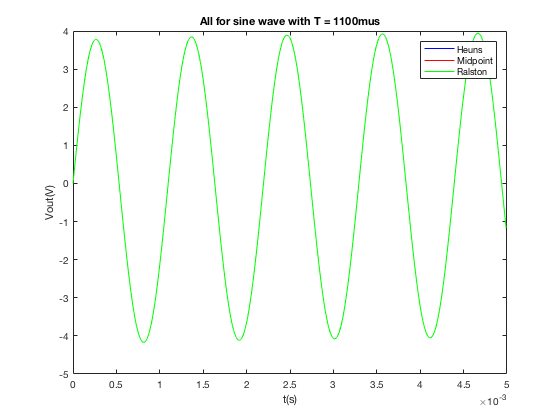
\includegraphics[width=.8\linewidth]{Ex1_Figs/allsine1100.png}
\caption{$T = 1100\mu s$,  h = 0.0000001 and tf = 0.00003}
\label{fig:sfig4}
\end{subfigure}
\caption{Plots of sine waves for different periods}
\label{fig:test4}
\end{figure}

%Put Comments on Figure 10 here



\FloatBarrier
\newpage
\subsubsection {Square wave with $\tilde{V}_{in} = 4V$}
   \begin{verbatim}
        vin = 4;
        T = ***10^(-6);
        t = t0: T : tf;
        f = 1/T;
        Vin =@(t) vin*square(2*pi*f*t);
    \end{verbatim}

    \begin{figure}[h]
        \begin{subfigure}{.5\textwidth}
          \centering
          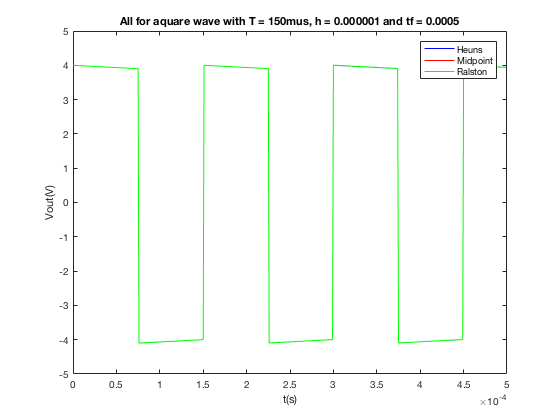
\includegraphics[width=.8\linewidth]{Ex1_Figs/square150.png}
          \caption{$T = 150\mu s$}
          \label{fig:sfig5}
        \end{subfigure}%
        \begin{subfigure}{.5\textwidth}
          \centering
          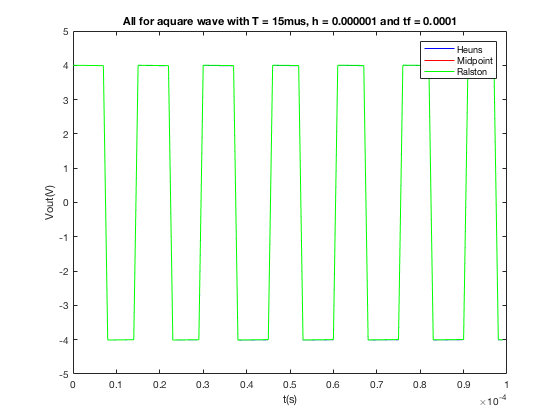
\includegraphics[width=.8\linewidth]{Ex1_Figs/square15.png}
          \caption{$T = 15\mu s$}
          \label{fig:sfig6}
        \end{subfigure}
        \begin{subfigure}{.5\textwidth}
          \centering
          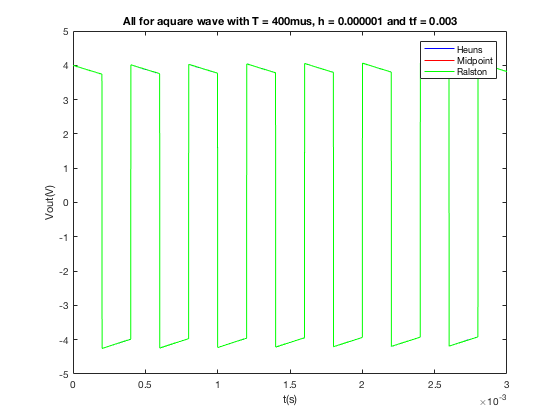
\includegraphics[width=.8\linewidth]{Ex1_Figs/square400.png}
          \caption{$T = 400\mu s$}
          \label{fig:sfig7}
        \end{subfigure}
        \begin{subfigure}{.5\textwidth}
          \centering
          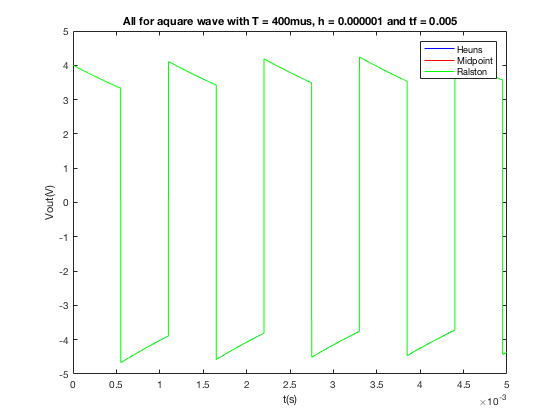
\includegraphics[width=.8\linewidth]{Ex1_Figs/square1100.png}
          \caption{$T = 1100\mu s$}
          \label{fig:sfig8}
        \end{subfigure}
        \caption{Plots of square waves for different periods}
        \label{fig:test5}
    \end{figure}


\newpage

\subsubsection{Sawtooth wave with $\tilde{V}_{in} = 4V$}

    \begin{verbatim}
        vin = 4;
        T = ***10^(-6);
        t = t0: T : tf;
        f = 1/T;
        Vin =@(t) vin*sawtooth(2*pi*f*t);
    \end{verbatim}

    \begin{figure}[h]
        \begin{subfigure}{.5\textwidth}
          \centering
          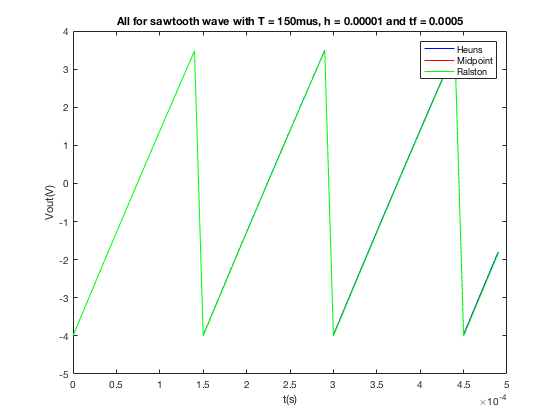
\includegraphics[width=.8\linewidth]{Ex1_Figs/sawtooth150.png}
          \caption{$T = 150\mu s$}
          \label{fig:sfig9}
        \end{subfigure}%
        \begin{subfigure}{.5\textwidth}
          \centering
          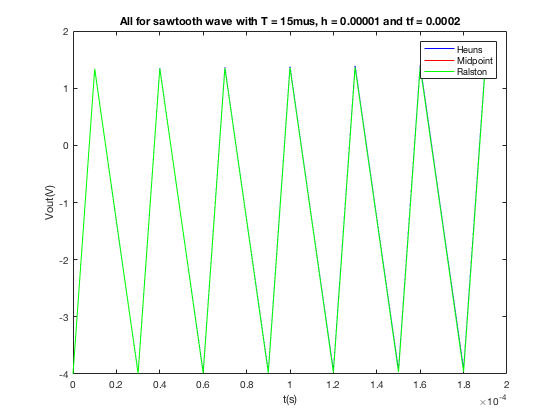
\includegraphics[width=.8\linewidth]{Ex1_Figs/sawtooth15.png}
          \caption{$T = 15\mu s$}
          \label{fig:sfig10}
        \end{subfigure}
        \begin{subfigure}{.5\textwidth}
          \centering
          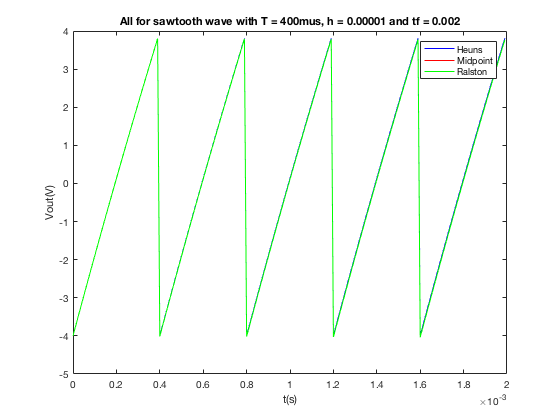
\includegraphics[width=.8\linewidth]{Ex1_Figs/sawtooth400.png}
          \caption{$T = 400\mu s$}
          \label{fig:sfig11}
        \end{subfigure}
        \begin{subfigure}{.5\textwidth}
          \centering
          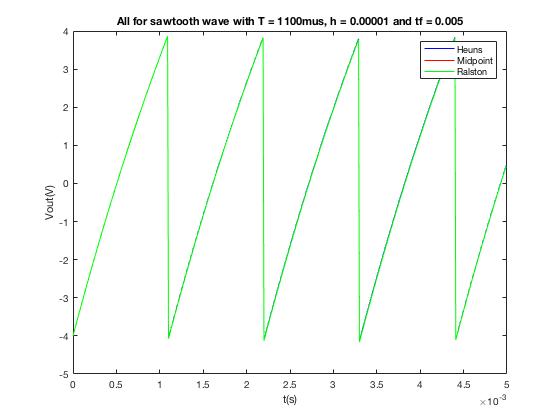
\includegraphics[width=.8\linewidth]{Ex1_Figs/sawtooth1100.png}
          \caption{$T = 1100\mu s$}
          \label{fig:sfig12}
        \end{subfigure}
        \caption{Plots of sawtooth waves for different periods}
        \label{fig:test6}
    \end{figure}

\pagebreak

\section{Exercise 2 - Error Analysis for RL Circuit}\vspace{-1mm}

\subsection{Background}

\vspace{-2mm}In Exercise 1, three numerical methods(Heun,Midpoint and Ralston) were used to estimate the value of functions for different inputs. However,these numerical methods have errors and do not give the exact solutions to the ODE. Therefore, in Exercise 2, the exact solutions to the ODEs will be obtained using MATLAB. These solutions will then be compared with those obtained using the numerical methods (in Exercise 1) to estimate the errors associated with the numerical methods.

\subsection{Exact Value}

For this RL circuit, a linear first order ODE is used to obtain the exact equation.

\subsection{Linear first order ODE}

\begin{equation}
\frac{dy}{dx}+p(x)y=Q(x)
\end{equation}

\begin{equation}
y(x)=Ce^{-\int{P(x)dx}}+e^{-\int{P(x)dx}}\int{Q(x)e^{\int{P(x)dx}}dx}
\end{equation}

\subsection{Linear first order ODE for RL circuit}

\begin{equation}
v_L(t)+v_R(t)=V_{in}(t)
\end{equation}
\begin{equation}
L\frac{di_L(t)}{dt}+Ri_L(t)=V_{in}(t)
\end{equation}

\begin{equation}
R=0.5\Omega
L=1.5mH
\end{equation}

Input is given as:

\begin{equation}
V_{in}=6cos(\frac{2{\pi}t}{150*{10^{-6}}})
\end{equation}

According to linear first order ODE, we get:

\begin{equation}
1.5*10^{-3}\frac{di_L(t)}{dt}+0.5i_L(t)=6cos(\frac{2{\pi}t}{150*{10^{-6}}})
\end{equation}

\begin{equation}
\frac{di_L(t)}{dt}+\frac{1}{3}*10^3i_L(t)=4*10^3cos(\frac{2{\pi}t}{150*{10^{-6}}})
\end{equation}

\begin{equation}
e^{{\frac{1}{3}*10^3}t}\frac{di_L(t)}{dt}+e^{{\frac{1}{3}*10^3}t}*\frac{1}{3}*10^3i_L(t)=e^{{\frac{1}{3}*10^3}t}*4*10^3cos(\frac{2{\pi}t}{150*{10^{-6}}})
\end{equation}

\begin{equation}
\frac{d(e^{{\frac{1}{3}*10^3}t}i_L(t))}{dt}=e^{{\frac{1}{3}*10^3}t}*4*10^3cos(\frac{2{\pi}t}{150*{10^{-6}}})
\end{equation}

Integrate both sides of the equation:

\begin{equation}
exact=-\frac{12}{1600\pi^2+1}exp(-1000/3t)+\frac{480\pi}{1600\pi^2+1}sin(\frac{40000t\pi}{3})+\frac{1}{1600\pi^2+1}cos(\frac{40000t\pi}{3})
\end{equation}

\subsection{Error Functions}
Using the same MATLAB scripts in Exercise 1 (heun.m,midpoint.m and ralston.m) the estimated values for the ODEs can be obtained. The result of subtracting these estimated solutions from the exact solutions leads to the error functions. In this section, the error functions will be developed using this technique for the three numerical analysis methods.

\subsubsection{Heun's Method}

\begin{figure}[h]
    \centering
    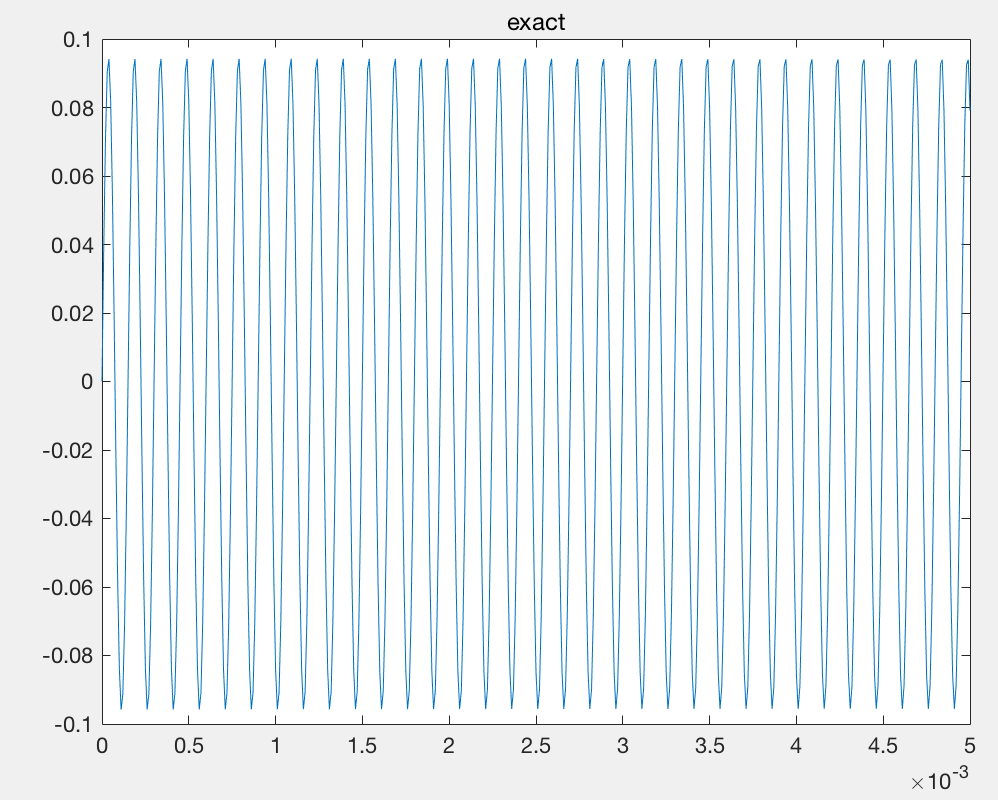
\includegraphics[scale=0.5]{Ex2_Figs/heun_error_exact}
    \caption{Exact Value}
    \label{fig:Exact Value}
\end{figure}

Figure \ref{fig:Exact Value} shows the exact solution to the ODE. Figure \ref{fig:Heun Method} shows the estimated solution using Heun's method. When the estimated solution is subtracted from the exact solution, the resulting function is the error function for Heun's method which is plotted in figure \ref{fig:heun_error}.

\begin{figure}[h]
\begin{subfigure}{.5\textwidth}
  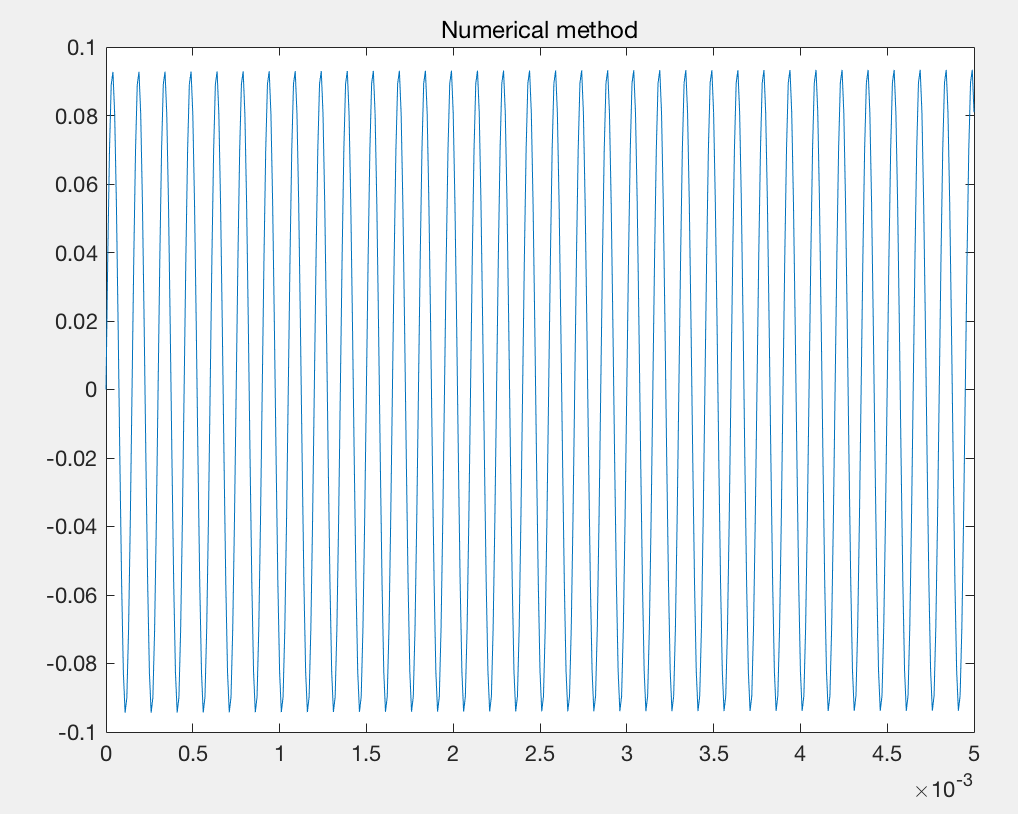
\includegraphics[width=.9\linewidth,height = 5cm
  ]{Ex2_Figs/heun_error_numerical_method}
  \caption[right]{Heun's Method}
  \label{fig:Heun Method}
\end{subfigure}
\begin{subfigure}{.5\textwidth}
  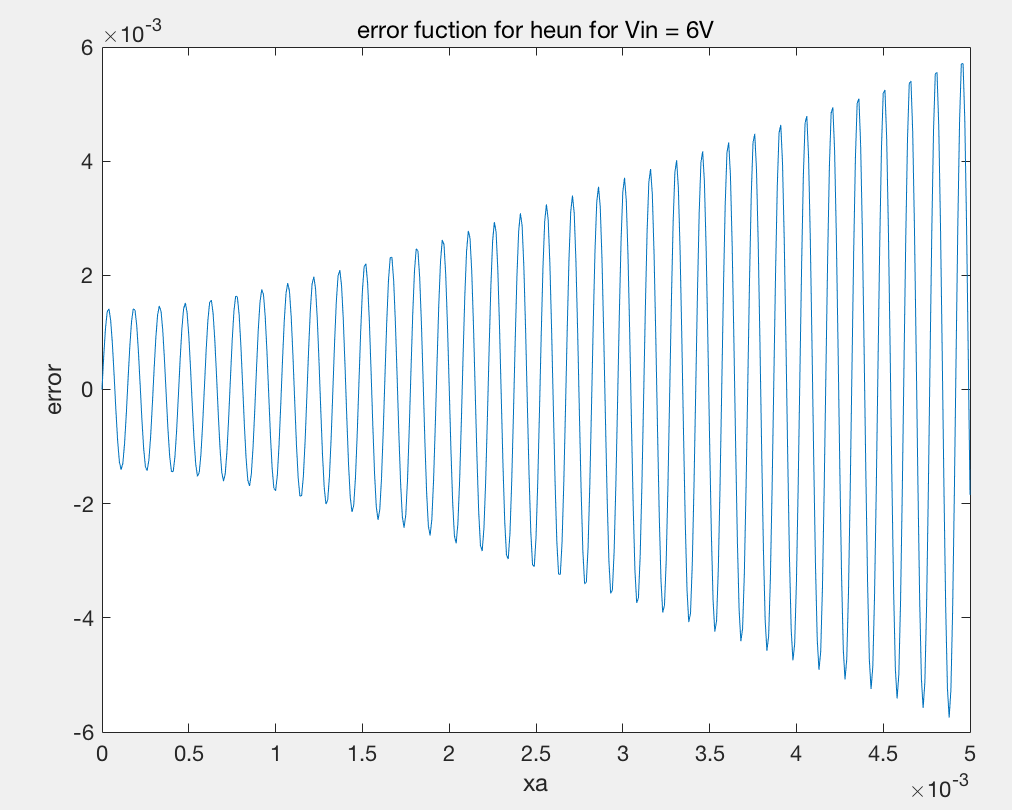
\includegraphics[width=.9\linewidth,height = 5cm]{Ex2_Figs/heun_error}
  \caption{Error function for Heun's Method}
  \label{fig:heun_error}
\end{subfigure}
\caption{Estimated solution and Error Function for Heun's method}
\label{fig:Heun_Error_sub}
\end{figure}



%% Add comments on the error function for Heun's method.


\clearpage

\subsubsection{Midpoint method}
The same analysis is used to obtain the error function for Midpoint method. The exact solution for the ODE is the same as that for Heun's method (Figure \ref{fig:Exact Value}).  Figure \ref{fig:midpoint_method} shows the estimated solution obtained by using the midpoint method. Similar to Heun's error analysis, when the estimated solution is subtracted from the exact solution, the resulting function is the error function. This error function is plotted in figure \ref{fig:midpoint_error}.

\begin{figure}[h]
\begin{subfigure}{.5\textwidth}
  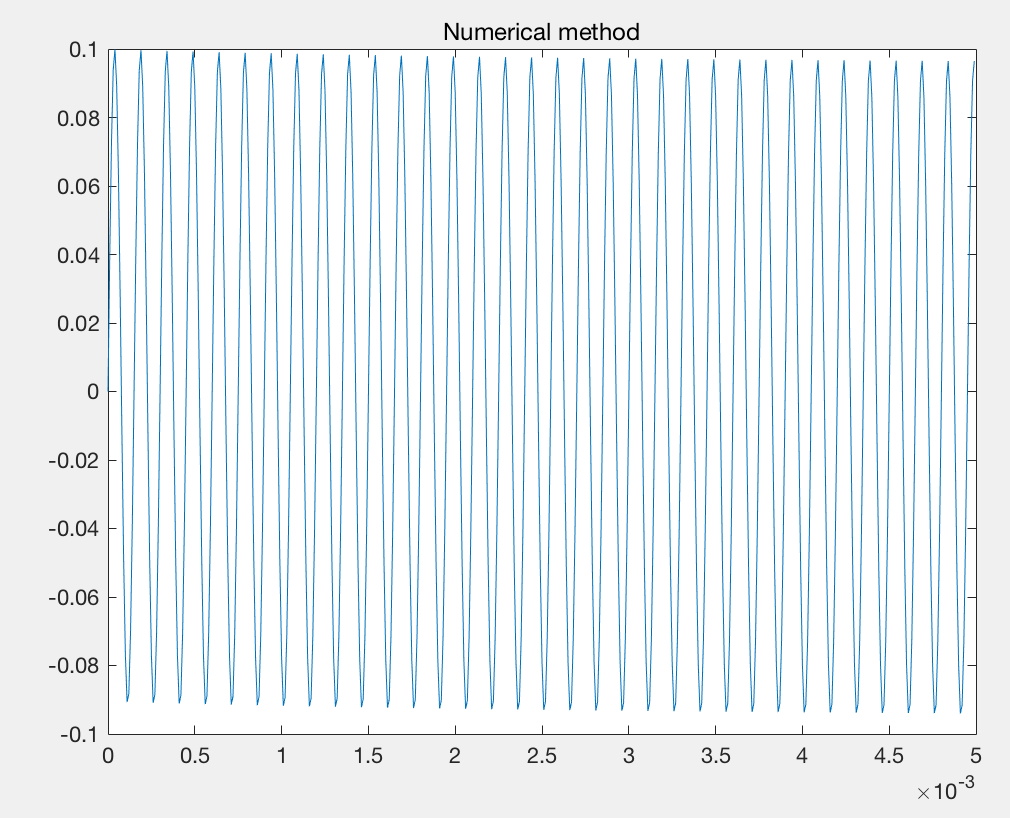
\includegraphics[width=.9\linewidth,height = 5cm
  ]{Ex2_Figs/midpoint_error_numerical_method}
  \caption[right]{Midpoint Method}
  \label{fig:midpoint_method}
\end{subfigure}
\begin{subfigure}{.5\textwidth}
  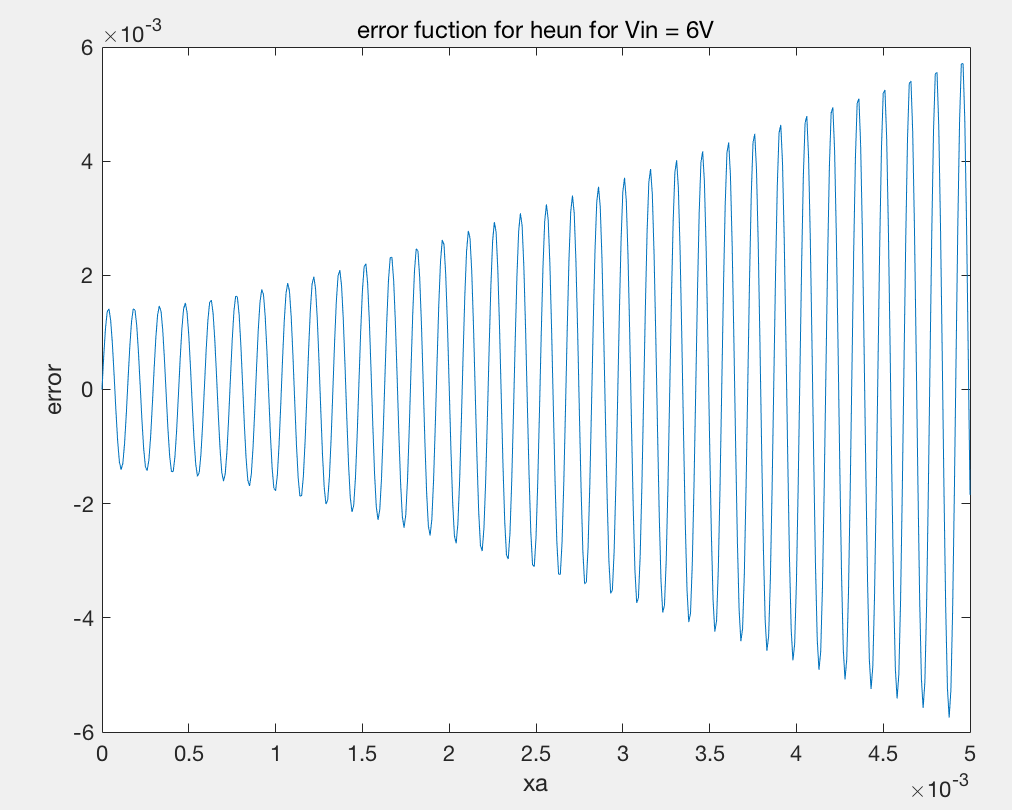
\includegraphics[width=.9\linewidth,height = 5cm]{Ex2_Figs/heun_error}
  \caption{Error function for Midpoint Method}
  \label{fig:midpoint_error}
\end{subfigure}
\caption{Estimated solution and Error Function for Midpoint method}
\label{fig:Method_Error_sub}
\end{figure}

%%Add comments on the error function for Midpoint here



\subsubsection{Ralston method}
Making use of the same error analysis technique as above (for Heun's and Midpoint methods), the estimated value obtained using the Ralston method is in figure \ref{fig:ralston_method} and the error function is plotted in figure \ref{fig:ralston_error}.

\begin{figure}[h]
\begin{subfigure}{.5\textwidth}
  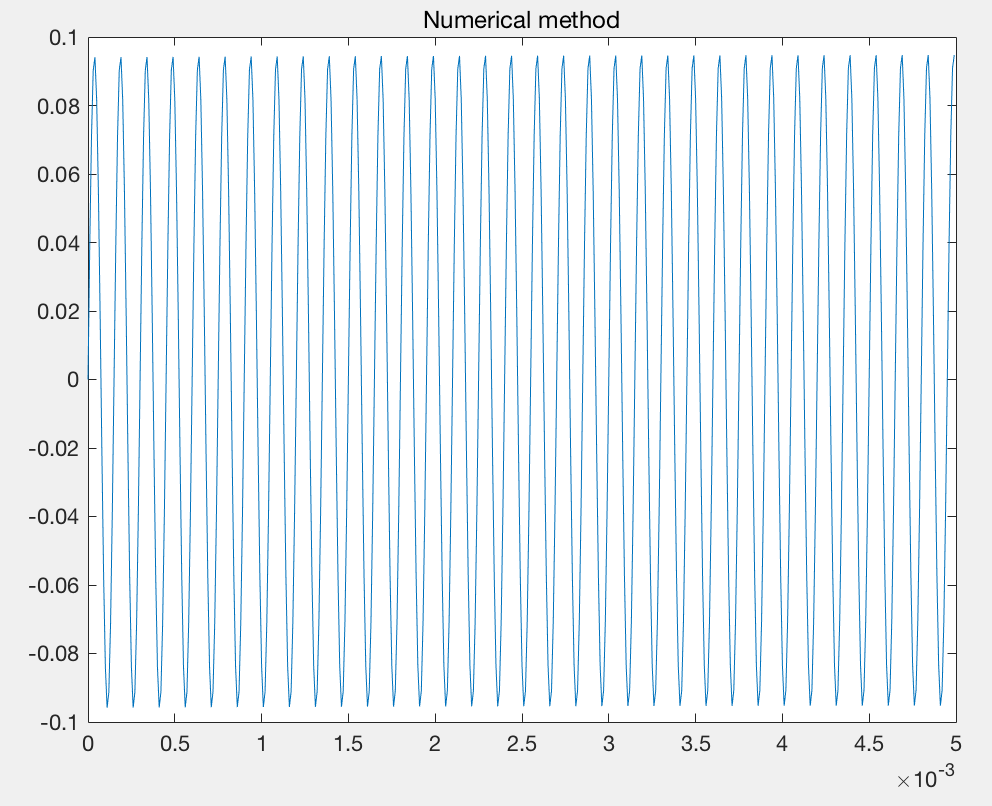
\includegraphics[width=.9\linewidth,height = 5cm
  ]{Ex2_Figs/ralston_error_numerical_method}
  \caption[right]{Ralston Method}
  \label{fig:ralston_method}
\end{subfigure}
\begin{subfigure}{.5\textwidth}
  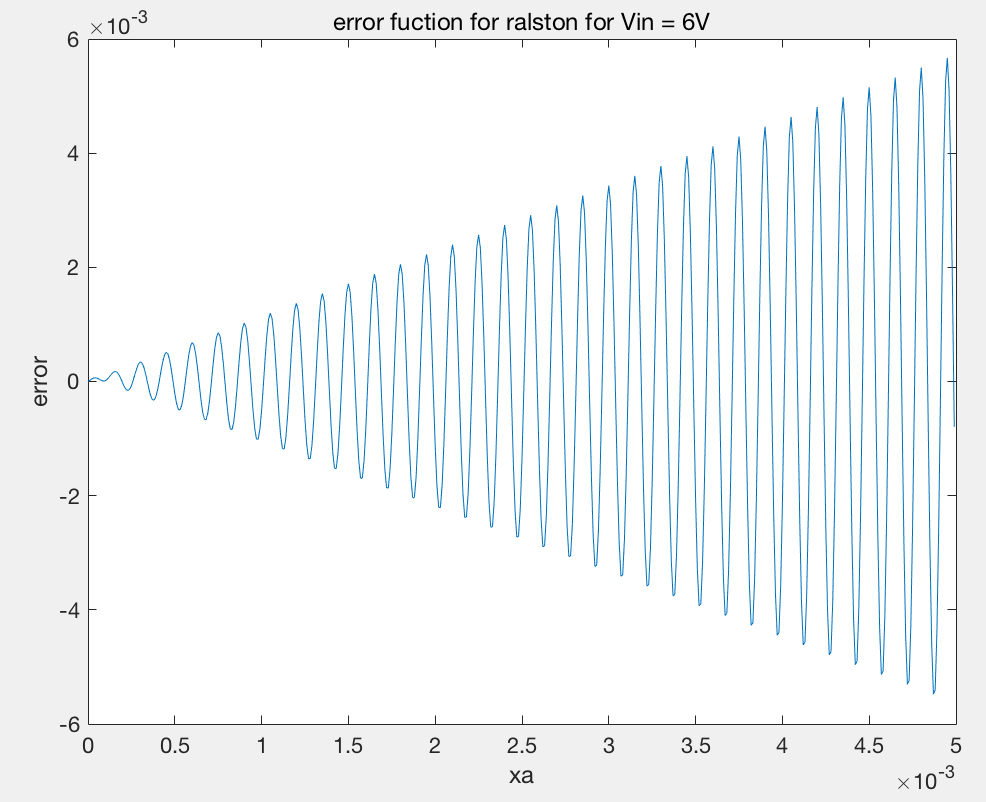
\includegraphics[width=.9\linewidth,height = 5cm]{Ex2_Figs/ralston_error}
  \caption{Error function for Ralston Method}
  \label{fig:ralston_error}
\end{subfigure}
\caption{Estimated solution and Error Function for Ralston method}
\label{fig:Ralston_Error_sub}
\end{figure}


%%Add comments on Ralston error function here

\clearpage

\subsection{Comparison}
For Heun's error function, the error increases from
$\underline{+}1.1*10^{-3}$ at 0 to $\underline{+}5.9*10^{-3}$ at $5*10^{-3}$. For the Midpoint error function, the error icreases from [-0.01,0] at 0 to [-0.011,0.01] at $5*10^{-3}$.
Finally, for Ralston's error function the error increases from 0 at 0 to $\underline{+}5.9*10^{-3}$ at $5*10^{-3}$.

Therefore, we can deduce that the Ralston method has the least error in approximating solutions for the linear first order ODE. %%Is this true?

\subsection{Log-log plot}
\begin{figure}[h]
    \centering
    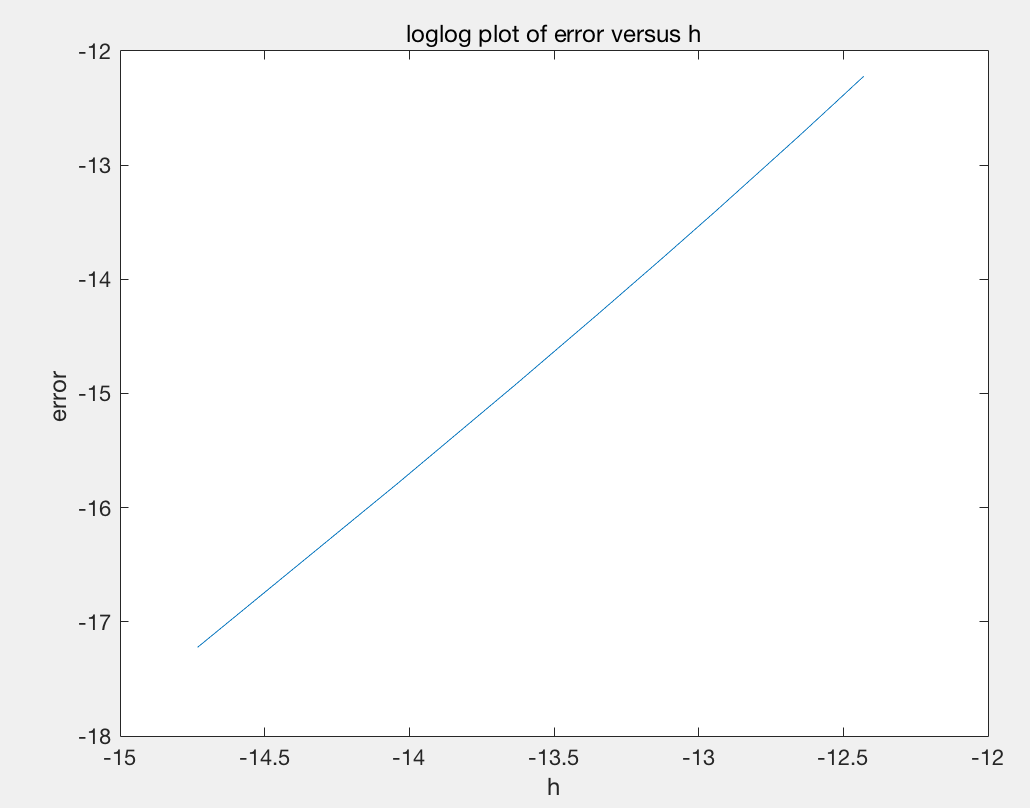
\includegraphics[scale=0.5]{Ex2_Figs/errorloglogfinal1}
    \caption{Log-Log plot for Ralston method}
    \label{fig:heun_error_loglog} %%heun's or ralston's?
\end{figure}

From figure \ref{fig:heun_error_loglog},it can be seen that as h increases, the error in the estimated solution using Ralston's method increases. Furthermore, the error has a positive linear relationship with h. The gradient of the straight line is approximately 2. It can be expressed as:

\begin{equation}
logE=2log(h)+constant
\end{equation}

Thus,it can be deduced that

\begin{equation}
E(y,x)=O(h^2);
\end{equation}



\pagebreak
\section{Exercise 3 - RLC Circuit}\vspace{-1mm}
\subsection{Background}

\begin{wrapfigure}{r}{0.5\textwidth}
\vspace{-10mm}
  		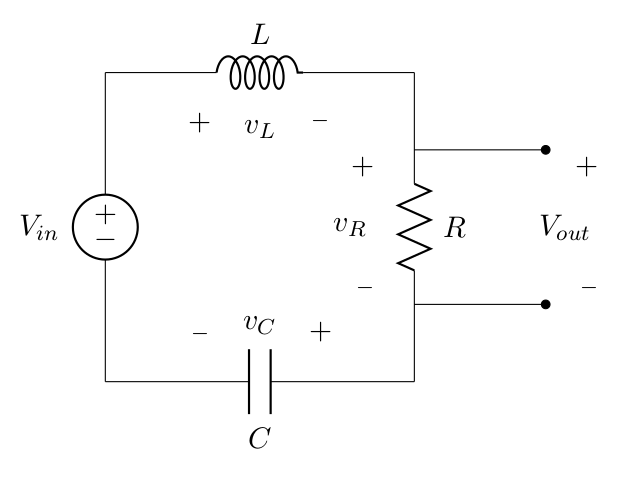
\includegraphics[width=0.49\textwidth]{Ex3_Figs/RLC.png}
\vspace{-6mm}
  	\caption{RLC Circuit}
  	\label{fig:RLC}
\end{wrapfigure}

%REMEMBER TO CHANGE FIGURE NUMBERS

From Kirchoff's Voltage Law (KVL) the sum of all the voltages in a closed loop must sum to 0 V. Therefore from this we can derive the equation $V_{in}(t) = v_L(t)+v_R(t)+v_C(t)$. All of the voltages in the closed loop current which flows through them, all being equal to the inductor current. The voltage across a conductor is the inductance multiplied by the derivative of it's current, the voltage across the resistor is equal to it's resistance multiplied by the current travelling through it and the voltage across the capacitor is the charge held within the capacitor divided by the capacitance of the capacitor. Substituting these characteristics into the equation above gives us the equation:

\[ L \frac{d}{dt}i_L(t) + R i_L(t) + \frac{1}{C}\int\limits_0^t i_L(t) \ dt = V_{in}(t)\]

Substituting $i_L(t)$ for $\frac{d}{dt}q_C(t)$ you make the equation:

\[ L \frac{d^2}{dt^2}q_C(t) + R\frac{d}{dt}q_C(t) + \frac{1}{C}q_C(t) = V_{in}(t)\]

We were then able to turn this second order ODE into a set of 2 coupled first order ODEs through the use of equating $q_C'(t)$ = $y(t)$ and substituting $q_C(t)$ for $x(t)$ we have the coupled equations:

\[y(t) = x'(t) \text{\hspace{5mm}and \hspace{5mm}}y'(t) = \frac{1}{L}[V_{in}(t)  - Ry(t) - \frac{1}{C}x(t)] \]

For our project we have values:

\[R = 250 \Omega, C = 3 \mu F , L = 650 mH, i_L(0) = 0 \hspace{2mm} (y_0) \text{\hspace{2mm}and\hspace{2mm}} q_C(0) = 500nC \hspace{2mm} (x_0).\]

\subsection{Script Coupled Equations and Constants}

Now that we have these two equations we are able to implement them into MATLAB scripf called `RLC\_script.m' by defining them as:

\begin{verbatim}
R = 250; L = 650*10^-3; C = 3*10^-6; %Impedance values for the components
w1 = 2*pi*500; %frequency for the 500 Hz sinusoid
w2 = 2*pi*100; %frequency for the sinusoid
w3 = 2*pi*5; %frequency for the sinusoid
tc = 3*10^-6; %tau for the exponential decay input
y0 = 0; x0 = 500*10^-9; t0 = 0; %Initial conditions y = iL, x =qC and t = time
h = 0.00001; %step size
tf = 0.03; %final condition
Vin = @(t) 5;
func1 = @(x, y, t) y; %y = q'
func2 = @(x, y, t) (Vin(t) - R*y - x/C)/L; %the second coupled equation
\end{verbatim}

\subsection{4th Order Runge Kutta 3/8 Algorithm}
\subsubsection{Theory}

To now evaluate these coupled equations, we use the Runge Kutta 4th order 3/8 algorithm to use these two coupled equations to estimate the next point of the current $i_L$ and the charge $q_C$. The algorithm is:

\[f_1(x,y,t) = y \hspace{3mm} f_2(x,y,z) = \frac{1}{L}[V_{in}(t) - Ry - \frac{x}{C}]\]
\[k1_x = hf_1(x_i,y_i,t_i) \hspace{3mm} k1_y = hf_2(x_i,y_i,t_i)\]
\[k2_x = hf_1(x_i+\frac{k1_x}{3},y_i+\frac{k1_y}{3},t_i+\frac{h}{3}) \hspace{5mm} k2_y = hf_2(x_i+\frac{k1_x}{3},y_i+\frac{k1_y}{3},t_i+\frac{h}{3})\]
\[k3_x = hf_1(x_i-\frac{k1_x}{3}+k2_x,y_i-\frac{k1_y}{3}+k2_y,t_i+\frac{2h}{3}) \]
\[k3_y = hf_2(x_i-\frac{k1_x}{3}+k2_x,y_i-\frac{k1_y}{3}+k2_y,t_i+\frac{2h}{3})\]
\[k4_x = hf_1(x_i+k1_x-k2_x+k3_x,y_ik1_y-k2_y+k3_y,t_i+h) \]
\[k4_y = hf_2(x_i+k1_x-k2_x+k3_x,y_ik1_y-k2_y+k3_y,t_i+h)\]
\[x_{i+1} =x_i+\frac{k1_x+3k2_x+3k3_x+k4_x}{8} \hspace{3mm} y_{i+1} =y_i+\frac{k1_y+3k2_y+3k3_y+k4_y}{8}\]
\[t_{i+1} = t_i + h \hspace{3mm} \text{where h is time step}\]

The way that this works is it starts from a single point and calculates a gradient to the next point, using this it then creates another slope, this is then repeated twice more using the equations above and a weighting is given to each gradient, summed together and divided by the total weighting to scale it back to uniform size, from this we are able to estimate more accurately where the next point if going to go for this time step.

\subsubsection{Implementation}

To implement this into MATLAB we created a function called `RK4second.m' in which would take in the two functions and work out the k efficients for both x and y and from there, work out the next position of the x (charge) and y (current) coordinates.

\begin{verbatim}
function [xout, yout] = RK4second (xin, yin, h, tin, func1, func2)

	k1x = h*feval(func1, xin ,yin, tin); %approx consts for RK4th ord 3/8 Method
k1y = h*feval(func2, xin ,yin, tin);
	k2x = h*feval(func1, xin + k1x/3, yin + k1y/3, tin+h/3);
	k2y = h*feval(func2, xin + k1x/3, yin + k1y/3, tin+h/3);
	k3x = h*feval(func1, xin  - k1x/3 + k2x, yin - k1y/3 + k2y, tin+2*h/3);
	k3y = h*feval(func2, xin  - k1x/3 + k2x, yin - k1y/3 + k2y, tin+2*h/3);
	k4x = h*feval(func1, xin + k1x - k2x + k3x, yin + k1y - k2y + k3y, tin+h);
k4y = h*feval(func2, xin + k1x - k2x + k3x, yin + k1y - k2y + k3y, tin+h);

	xout = xin + (k1x + 3*k2x + 3*k3x + k4x)/8;
	yout = yin + (k1y + 3*k2y + 3*k3y + k4y)/8;
end
\end{verbatim}

This takes in the present value of current and charge a certain time, the time position, the step time and the two functions to evaluate and approximate the next point, which is then outputted at the end.

\subsection{RLC\_Script.m Implementation}

\begin{verbatim}
N = round((tf-t0)/h); %calculates number of time steps
ya = zeros(1,N); xa = zeros(1,N);
ta = zeros(1,N); in = zeros(1,N); %set up arrays

xa(1) = x0; ya(1) = y0; ta(1) = t0; in(1) = Vin(t0); %input initial conditions
for i = 1:N-1 %works out next timestep value
	   [xa(i+1), ya(i+1)] = RK4second (xa(i), ya(i), h, ta(i),func1, func2);
    ta(i+1) = ta(i) + h; %next time step
    in(i+1) = Vin(ta(i+1)); %next value of the input
end

figure; %sets up the figures
Vout = R*ya; %Vout = R*iL
subplot(2,1,1);
plot(ta, Vout); %plot output Voltage
grid on;
xlabel('Time/s'); ylabel('Voltage Out/V');
title('R*dq/dt with a Step Response')
subplot(2,1,2);
plot(ta, in); %plot input Voltage
grid on;
xlabel('Time/s'); ylabel('Voltage In/V');
title('Step Response')
\end{verbatim}

\subsection{Exercise 3 Graphs}
\subsubsection{Step Response}

\begin{wrapfigure}[13]{r}{0.46\textwidth}

	\vspace{-6mm}
  		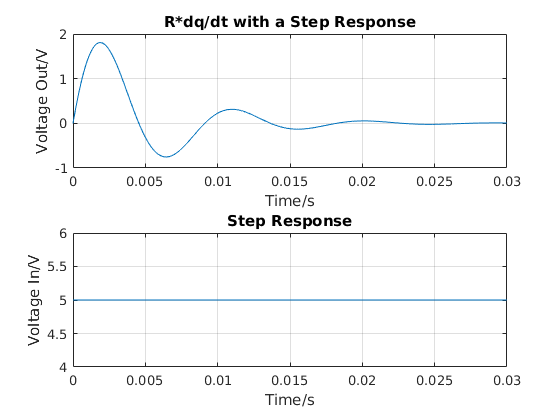
\includegraphics[width=0.45\textwidth]{Ex3_Figs/Step.png}
	\vspace{-6mm}
  	\caption{$V_{in}(t)= 5$}
  	\label{fig:ex3g1}

\end{wrapfigure}

    \vspace{0mm}The step response causes a sudden rise of voltage up to 5 V, due to the inductor not being able to change current instantaneously the voltage out starts from 0 V and as you can see on Figure 2. It increases up to around 1.8 V at this point the capacitor starts to reduce the rate of it charging up due to saturating in charge, as the voltage out starts to tend to 0, the capacitor emits charge causing a negative current through the inductor. As this goes on, the voltage across the capacitor tends to 5 V causing no current to flow through the inductor and the resistor, causing the output voltage to tend to 0 V.

\subsubsection{Sine Wave Input}

\begin{wrapfigure}[13]{r!}{0.46\textwidth}
    \vspace{-5mm}

  		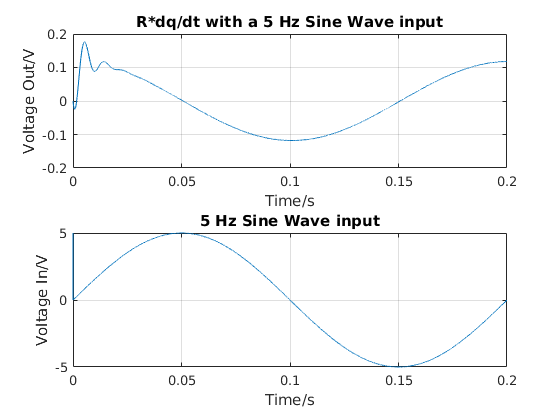
\includegraphics[width=0.45\textwidth]{Ex3_Figs/5Sine2.png}
	\vspace{-6mm}
  	\caption{$V_{in}(t)= 5sin(2 \pi 5t)$}
  	\label{fig:ex3g2}

\end{wrapfigure}

\vspace{0mm}In Figure 3 the input is a sine wave of amplitude 5 V and a frequency of 5 Hz, as the sine wave moves away from zero it causes a sharp increase in the current going through the inductor and therefore causes a sharp rise on the voltage out, this then attenuates to form the shape of a sine wave of amplitude is $\approx 0.1$ V and leads the input voltage by a phase difference of $\frac{\pi}{2}$ this is relative to the frequency of the input and the complex impedance of both the inductor and the capacitor being $j\omega L$ and $\frac{1}{j\omega C}$ respectively. We chose the final time as 0.2 s to show how initially the output changes but then follows the shape of the input eventually.

\begin{wrapfigure}[16]{r}{0.46\textwidth}
    \vspace{-15mm}
  		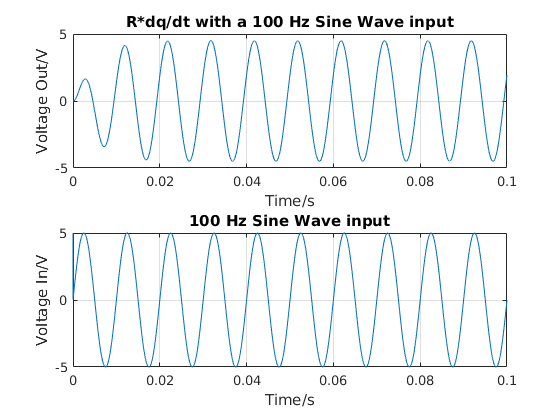
\includegraphics[width=0.45\textwidth]{Ex3_Figs/100Sine.png}
	\vspace{-6mm}
  	\caption{$V_{in}(t)= 5sin(2 \pi 100t)$}
  	\label{fig:ex3g3}
\end{wrapfigure}

\vspace{6mm}In Figure 4 the input is a sine wave of amplitude 5 V and a frequency of 100 Hz. Upon the start of the wave, the output voltage rises slower than the voltage of the input, due to the fact that the rate of change of the inductor current cannot shange instantaneously and will eventually equal the frequency of the input. This causes a slight phase difference and the amplitude is far greater than the 5 Hz input, resulting in an amplitude of $\approx 4$ V. This greater output voltage is due to being a band pass filter, low frequencies as we can see, 5 Hz for example attenuate to a value close to 0 V whereas at this frequency the output voltage is close to the input voltage and at some frequency greater than this, the same result as the 5 Hz wave will be apparent.

\begin{wrapfigure}[11]{r}{0.46\textwidth}
    \vspace{-33mm}
  		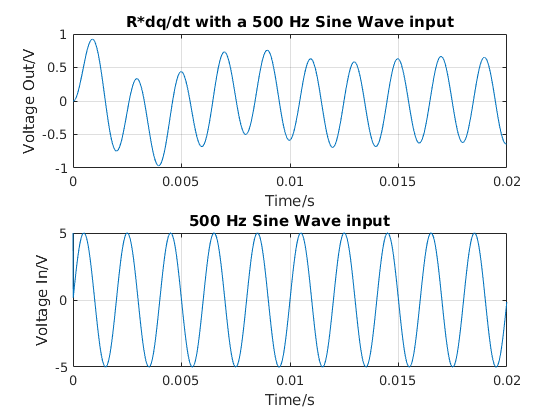
\includegraphics[width=0.45\textwidth]{Ex3_Figs/500Sine.png}
	\vspace{-6mm}
  	\caption{$V_{in}(t)= 5sin(2 \pi 500t)$}
  	\label{fig:ex3g4}
\end{wrapfigure}

\vspace{2mm}In Figure 5 the input is a sine wave of amplitude 5 V and a frequency of 500 Hz. The response is very similar to Figure 3's output signal, rising initially to a value that is greater than its steady state amplitude in which is $\approx 0.5$ V which is far 10 times less than the input amplitude, and less than the the amplitude of the Figure 4. This suggests that the center of the band pass filter is based around 100 Hz as is seen in Figure 4 and therefore the outer bounds falling in amplitude at frequencies greater and less than this.

\subsubsection{Square Wave Inputs}

\begin{wrapfigure}[11]{r}{0.46\textwidth}
    \vspace{-40mm}
  		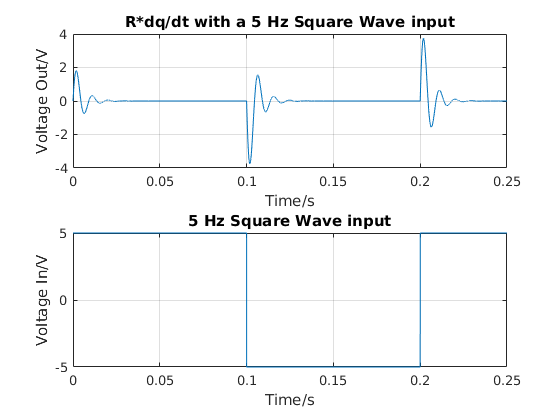
\includegraphics[width=0.45\textwidth]{Ex3_Figs/5Squ1.png}
	\vspace{-6mm}
  	\caption{$V_{in}(t)= 5square(2 \pi 5t)$}
  	\label{fig:ex3g5}
\end{wrapfigure}

\vspace{3mm}In Figure 6 the input is a square wave of frequency 5 Hz and amplitude 5 V. At this frequency, the response is identical to the response of a step response due to there being enough time for the wave to return to 0 V after the change in amplitude, the only difference is when the voltage drops to -5 V the step response is equal to the positive step response but negative. The time scale was chosen to show 1 and a quarter wavelengths so that it is easy to see that each time the sign changes, the response is identical.

\begin{wrapfigure}[8]{r}{0.46\textwidth}
    \vspace{-40mm}
  		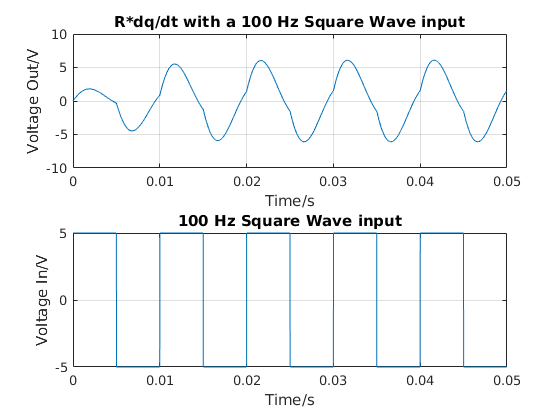
\includegraphics[width=0.45\textwidth]{Ex3_Figs/100Squ1.png}
	\vspace{-6mm}
  	\caption{$V_{in}(t)= 5square(2 \pi 100t)$}
  	\label{fig:ex3g6}
\end{wrapfigure}

\vspace{5mm}In Figure 7 the input is a square wave of frequency 100 Hz and amplitude 5 V. At this frequency, the output follows the characteristic of a sine wave due to the step response giving a sinusoidal peak, this is repeated but switched in direction as the sign of the input changes, causing a periodic signal on the output respresenting something somewhat similar to a sine wave.

\begin{wrapfigure}[17]{r}{0.46\textwidth}
    \vspace{-5mm}
  		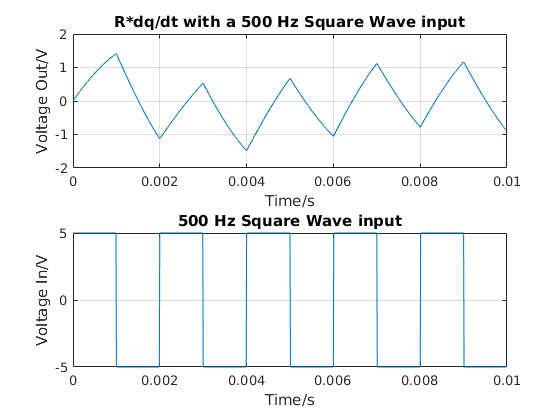
\includegraphics[width=0.45\textwidth]{Ex3_Figs/500Squ1.png}
	\vspace{-6mm}
  	\caption{$V_{in}(t)= 5square(2 \pi 500t)$}
  	\label{fig:ex3g7}
\end{wrapfigure}

\vspace{5mm}In Figure 8, the input is a square wave of frequency 500 Hz and amplitude 5 V. At this frequency, the step responses cause an output signal which is similar to a periodic tent function of exponential charge and discharge, this is due to the fact that the square wave changes sign too rapidly for the signal to smooth off or return to zero before the next half wavelength. As it gets to the 4th period of the input, the output settles to an amplitude of $\approx 1$ V. In which looking back over Figures 6, 7 and 8. The bandpass filter seems to give similar changes in output amplitude relative to the input amplitude, where at 100 Hz, in Figure 7 the magnitude is greater than both magnitudes. Confirming that the center frequency if based around 100 Hz and the bandwidth is based between 5 Hz and 500 Hz.

\subsubsection{Exponential Decay Input}

\begin{wrapfigure}[9]{r}{0.46\textwidth}
    \vspace{-23mm}
  		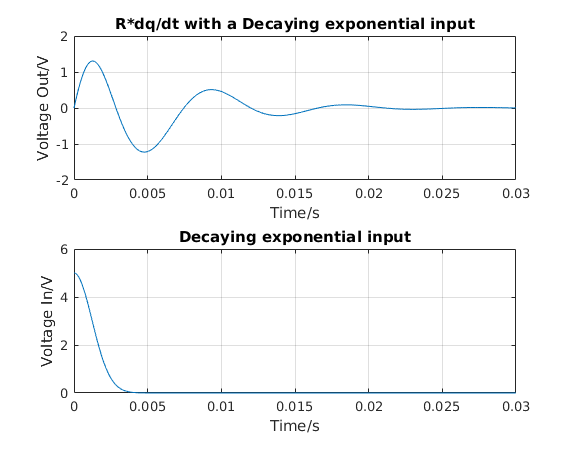
\includegraphics[width=0.45\textwidth]{Ex3_Figs/DecExp.png}
	\vspace{-6mm}
  	\caption{$V_{in}(t)= 5e^{\frac{-t^2}{\tau_C}}$}
  	\label{fig:ex3g8}
\end{wrapfigure}

In Figure 9, the input is a decaying exponential in which it's time constant $\tau_C = 3 (ms)^2$ causing a sharp drop in amplitude towards 0 V in a time of less than 5 ms, causing an output in which is incredibly similar to the output of the step responss (Figure 2). The only main difference being that the max amplitude of the output of Figure 9 is $\approx 1$ V, $\approx 0.8$ V less than the max amplitude of Figure 2 in which the amplitude was $\approx 1.8$ V.

\pagebreak

\section{Exercise 4 - Finite Differences for PDE}\vspace{-1mm}
\subsection{Background}

For this exercise we were asked to implement the finite difference method for the 1D heat equation which is:

\[\frac{\partial y}{\partial t} = \frac{\partial^2 x}{\partial t^2}\ \hspace{5mm} \text{in which} \hspace{5mm} 0 < x < 1, \hspace{5mm} t > 0 \hspace{5mm} \text{and} \hspace{5mm} y(0,t) = y(1,t) = 0 \hspace{2mm} \forall \hspace{2mm} t\]

\subsection{Script Equations and Constants}

\begin{verbatim}
x0 = 0;
h = 0.005; %Step size in the X direction
Tin = @(x) sin(2*pi*x);
Bc = @(t) 0;
xf = 1 + h; %Final value of X plus one more step to complete the graph
t0 = 0; %Initial time value
k = 0.45*h^2; %v max of 1/2 we use 0.45 work out k relatively, steps in time
tf = 200*k; %the end time is 250 steps in the k direction
N = round((xf-x0)/h); %number of steps in the x direction
M = round((tf - t0)/k); %number of steps in the t direction
v = k/(h^2); %recalculating the value of v
b = 1 - 2*v; %create the value of beta
ya = zeros(1,N); xa = zeros(1,N); %create empty arrays
xa(1) = x0; xa(N) = xf-h;  ya(1) = Bc(0); ya(N) = Bc(0); %initial conditions
\end{verbatim}

In the script above, we define the step size in the x direction, from this we are then able to calculate k, the step in time. Due to the formula to calculate finite difference:

\[U^{m+1}_j = vU^m_{j-1} +(1-2v)U^m_{j}+vU^m_{j+1} \hspace{5mm} \text{where for stability} \hspace{5mm} v < \frac{1}{2}\]

Therefore by making v = 0.45, thus never becoming unstable, if the x direction step size is changes, we can calculate k by multiplying it by $h^2 \hspace{5mm} \text{due to} \hspace{5mm} v = \frac{k}{h^2} \hspace{5mm} \text{we also replaced} \hspace{2mm} 1-2v \hspace{2mm} \text{with} \hspace{2mm} \beta $.

\subsection{Implementation of the Finite Difference Method}

\begin{alltt}
for i = 1:N-2
    xa(i+1) = xa(i) + h; %next step in x direction
    ya(i+1) = feval(Tin, xa(i+1)); %calculate heat inital points
end
t = t0; %initial time value
plot(xa, ya, '.', 'markersize', 4); %plot graph at t = 0
hold on; %plots them all on the same graph
yn = ya; %to take the next time values
for a = 1:15 %plots the graph 15 times
    for i = 1:M %cycle through every time step
        ya(1) = Bc(t); ya(N) = Bc(t); %set boundary conditions
	       for j = 2:N-1 %work out temp for next time step
           yn(j) = v*ya(j-1) + b*ya(j) + v*ya(j+1);
	       end
        t = t+k; %change the time one step forward
        ya = yn; %replace ya with the next time array
    end
    plot(xa, ya, '.', 'markersize', 4); %plot heat
    title 'Finite Difference of PDE 1D Heat Equation - '
end
xlabel 'Distance/cm'
ylabel 'Temperature/C'
\end{alltt}

The way that it works is that we use a for loop to calculate the initial temperature value at each spot on the x axis and place them into the array ya, this then is plotted on a graph to show the initial graph. After that we then use a for loop which runs 15 times so that we are able to plot each graph whilst being able to visualise how it changes as time increases. There is then another for loop in which cycles through every step, in which recalculates the boundary conditions (for the sake of having a time variable boundary conditions). Finally within another for loop it cycles through all the points between the first and last values of temperature and using the finite difference equation stated above. After this ya is replaced with the new calculated array and then the values are plotted on the graph.

\subsection{Finite Difference Graphs}

\begin{wrapfigure}[28]{r}{0.50\textwidth}
    \vspace{-13mm}
  		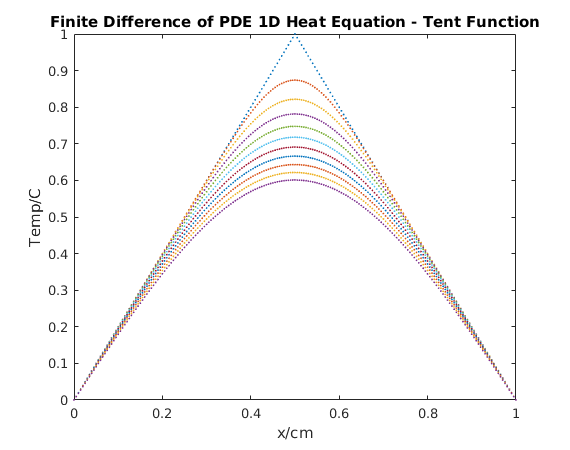
\includegraphics[width=0.45\textwidth]{Ex4_Figs/FiniteTent.png}
	\vspace{-4mm}
  	\caption{$T_{in}(x)= tent(x)$}
  		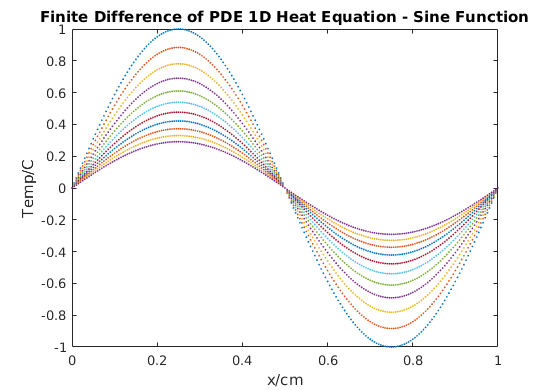
\includegraphics[width=0.45\textwidth]{Ex4_Figs/FiniteSine.png}
	\vspace{-4mm}
  	\caption{$T_{in}(x)= sin(2{\pi}x)$}
    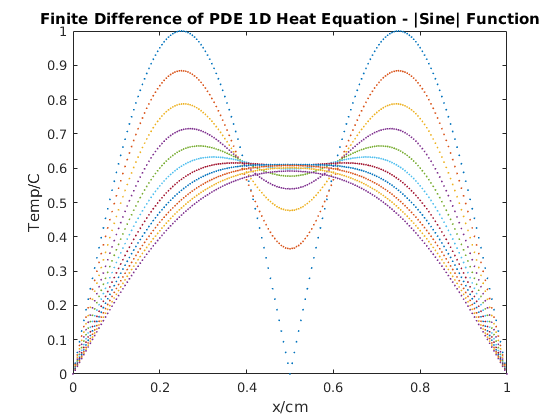
\includegraphics[width=0.45\textwidth]{Ex4_Figs/FiniteSineabs.png}
    \vspace{-4mm}
    \caption{$T_{in}(x)= |sin(2{\pi}x)|$}
  	\label{fig:ex4g1}
\end{wrapfigure}

As is shown in Figure 10, for the tent function the temperature decreases as it tends towards 0 and 1 from the centre of 0.5. As it steps through time, the heat tries to diffuse evenly within the object, this is shown by as time goes on, the heat decreases within the body and if we were to go further into time, the heat would altogether tend to zero across the body.

\vspace{3mm}In Figure 11 you can see the sine function in which meets the boundary conditions, having `positive' and `negative' temperatures, they have identical characterisics of how the temperature is dissipated. The central point at x = 0.5 remains equal to 0 due to the equation taking both points either side of it and multiplying with v, in which they both have the same magnitude, but different signs so when added together they cancel and cause the temperature to remain at 0 for the time being.

\vspace{3mm}In Figure 12, the absolute value of the sine wave was taken in which the reason it differs with the standard sine curve is that due to now across the centre, on either side the point they are no longer opposite in magnitude, therefore the point at the centre increases in magnitude as the heat disperses across the body, trying to uniformally distribute it.

\pagebreak

\begin{wrapfigure}[15]{r!}{0.5\textwidth}
	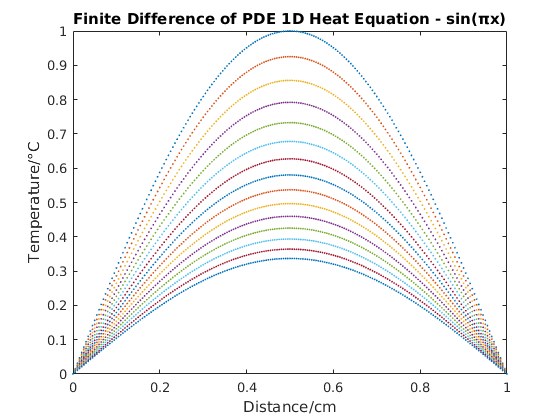
\includegraphics[width=0.45\textwidth]{Ex4_Figs/sinpi.png}
	\vspace{-3mm}
	\caption{$T_{in}(x)= sin(\pi x)$}
	\label{fig:test1}
		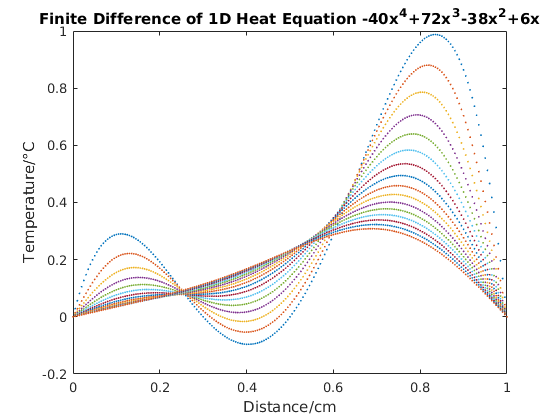
\includegraphics[width=0.45\textwidth]{Ex4_Figs/poly.png}
		\vspace{-3mm}
	\caption{$T_{in}(x)= -40x^4 +72x^3 -38x^2 +6x$}
	\label{fig:test2}
\end{wrapfigure}

In Figure 13, the input is half of a sine wave in which you can simply see as time goes on, throughout the body, the heat dissipates, tending towards 0.

\vspace{4mm}In Figure 14, the input is a polynomial with the roots $x$ = 0, 0.3, 0.5 and 1 showing a very random distribution of the heat throughout the body, at the start of time, the heat from $0 < x < 0.5$ smooths off a lot quicker than  the second half of the graph due to the fact that there is a maximum at the point of $x \approx 0.83$ this takes a while for the heat to dissipate. As with all the rest, as time travels towards infinity, the heat will tend to 0, unifomally across the body.

\vspace{40mm}
\subsection{Bonus Exercises}
\subsubsection{Boundary Conditions Not Met}

\begin{wrapfigure}[21]{r!}{0.5\textwidth}
	\vspace{-10mm}
	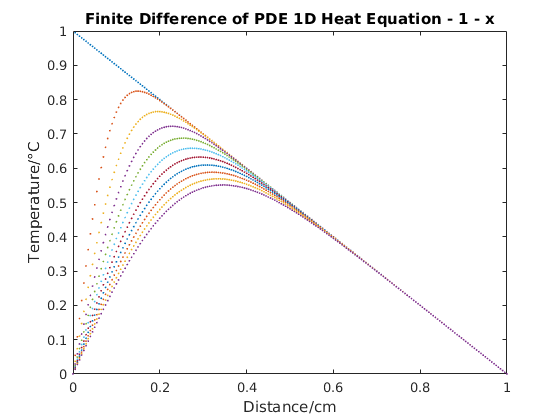
\includegraphics[width=0.45\textwidth]{Ex4_Figs/1-xbcdiff.png}
	\vspace{-3mm}
	\caption{$T_{in}(x)= 1-x$}
	\label{fig:bcnm}
		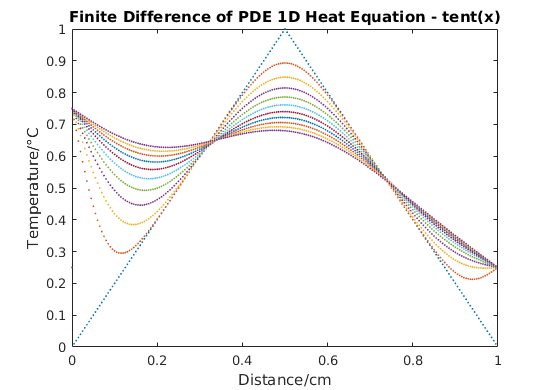
\includegraphics[width=0.45\textwidth]{Ex4_Figs/Tentbc.png}
		\vspace{-3mm}
	\caption{$T_{in}(x)= tent(x) \hspace{2mm} y_0(t) = 0.75, y_1(t) = 0.25$}
	\label{fig:bmsn2}
\end{wrapfigure}

In Figure 15, the input was the straigt line of $T_in(x) = 1-x$ where the left hand portion of the graph doesn't meet the left hand condition. With the boundary condition both being 0, it causes the temperature from just after x = 0 to fall away considerably quicker than any other portion of the graph due to the greater difference the boundary condition and the points to the side of it, as you can see on Figure 15.

\subsubsection{Non Zero Boundary Conditions}

In Figure 16, the input is a tent function, but rather than having boundary conditions in which were equal to 0, the boundary condition at x = 0, the temperature is equal to 0.75 and at x = 1, the value is equal to 0.25. As you can see the points to the left of the graph all pull up towards the value of 0.75 and on the other side, all the points are pulled towards the 0.25. As time goes to infinity, you would get the heat distributed as a straight line going from 0.75 to 0.25.

\pagebreak

\subsubsection{Time Varying Boundary Conditions}

\begin{wrapfigure}[10]{r!}{0.5\textwidth}
	\vspace{-6mm}
	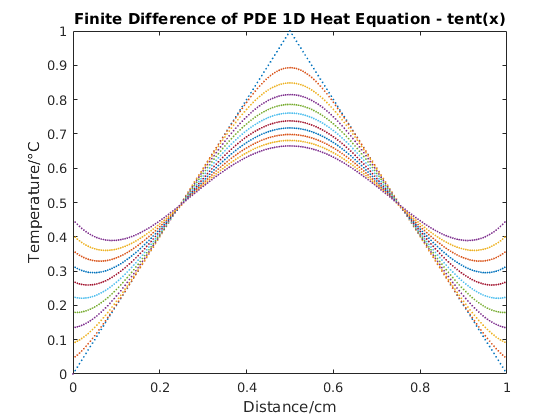
\includegraphics[width=0.45\textwidth]{Ex4_Figs/timevar.png}
	\vspace{-3mm}
	\caption{$T_{in}(x)= tent(x) \hspace{2mm} y_0(t) = y_1(t) = 20t$}
\end{wrapfigure}

In Figure 17, the input is a tent function, initially with zero boundary conditions, but as time moves forward, the temperature at the end points increases with the equation of $y_0(t) = y_1(t) = 20t$. So the heat in the body will end up heating up from the edges inwards.

\end{document}
